\chapter[Metodologia]{METODOLOGIA}
\label{ch:cap3}

Nesta seção, será apresentada de forma técnica e descritiva a metodologia utilizada para o desenvolvimento da ténica de compressão de redes neurais profundas por poda, análise dos resultados obtidos de acurácia e esparsidade para modelos sem utilização de poda e para podas mais agressivas.

A metodologia adotada para realizar os primeiros experimentos foi, inicialmente, a seleção dos dados a serem utilizados para classificação, definição do modelo de rede e definição das bibliotecas e o ambiente de desenvolvimento a ser utilizado. Após isso, foram definido os hiperparametrose as métricas a serem analisadas para os resultados obtidos. E então, o processo de aprendizagem foi realizado.

%O processo de aprendizagem foi realizado com os mesmos parâmetros sete vezes, sendo modificado apenas o valor de $ \alpha $, que define o quão agressiva é a poda. Além disso, também é computada a quantidade de pesos que foram removidos para o cáculo da esparsidade do modelo.

%Por fim, foram análisados os resultados obtidos, levando em consideração a quantidade de pesos significativos através da esparsidade final do modelo e a acurácia obtida. Com esses resultados, é possível montado a rede neural no hardware com a mesma estrutura e pesos do modelo treinado, removendo os pesos insignificantes.


%\begin{itemize}
%    \item Primeiro
%    \subitem - $C_1 > F_1 + F_2 $
%    \item Segundo
%    \subitem - $C_2 > F_1 + F_2 - C_1$
%\end{itemize}

%\begin{equation} \label{eq1}
%R(t) = P(T > t) = 1 - F(t)
%\end{equation}

\section{Proposta} \label{secao1}

Uma das características das redes neurais é a grande quantidade de operações numéricas realizadas durante os processos de treinamento e inferência. Nos hardwares, em geral, muitas operações matemáticas aumentam significativamente o seu consumo energético. Como resultado, aparelhos alimentados por bateria ainda não conseguem executar redes neurais convolucionais de ultima geração devido o seu limite energético \cite{yang2017}.

As técnicas de compressão mais convencionais realizam a poda somente no primeiro batch de cada época, ou ao final de cada época. A proposta é a realização da poda em todos os batches. A aplicação desta técnica já foi utilizada para classificação viral \cite{fernandes2021}, a proposta é utilizar a mesma ténica para classificação de imagens.


\subsection{Treinamento} \label{secao11}

A estratégia escolhida para redução da quantidade de operações númericas foi a de compressão por poda. Assim, durante o treinamento, foi aplicada a poda em todas as camadas do modelo baseados em um limiar ($ \beta_k $) definido pelo desvio padrão dos seus pesos multiplicados por uma constante $ \alpha_k $ determinada antes do processo de treinamento. Esta variável é que indica o quão agressiva será a compressão do modelo. Todos os pesos com magnitude menor que esse valor são removidos. 

O processo de aprendizado e compressão por poda pode ser vizualizado na Figura 10. Onde $Y(n)$ é a classe predita pelo modelo para a entrada $X(n)$. O erro $E(n)$ é calculado a partir da diferença entre a saída predita e $Y_{ref}(n)$ que é a classe real do dado de entrada. A partir do erro, é claculado o gradiente de descida $G(n)$ e então os pesos são atualizados. $C(n)$ são os pesos do modelo após o processo da poda. Os pesos que foram zerados também passam pelo cálculo do gradiente.

\begin{equation}
    \beta_k = \alpha * \sigma_k
\end{equation}

\begin{equation}
    C_k(n) = P(W_k(n),\beta_k) =
    \begin{cases}
      w_k(n) & \text{if } |w_k(n)|\geq \beta_k \\
      0 & \text{if } |w_k(n)| < \beta_k\\
    \end{cases} 
\end{equation}

A Equação 3.1 mostra como é feito o cálculo do limiar, sendo $ \beta_k $ o limiar da \textit{k}-ésima camada, $\alpha$ a constante que estabelece a agressividade da poda e $\sigma_k$ o desvio padrão da \textit{k}-ésima camada.

Na Equação 3.2 temos P(.,.), que representa a função de poda, é feita a análise se o \textit{n}-ésimo peso da \textit{k}-ésima camada é menor que o limiar calculado. Se for, o valor do peso passa a ser zero. As Figuras 12 e 13 apresentam um exemplo da remoção dos pesos para $ \alpha $ = 0.75, removendo um total de 15638 parâmetros dessa camada.

\begin{figure}[!h]
    %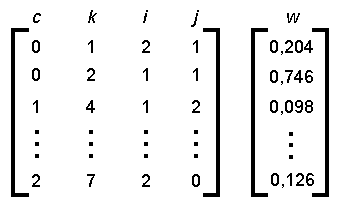
\includepdf[pages=-, width=6cm]{figuras/figx.pdf}
	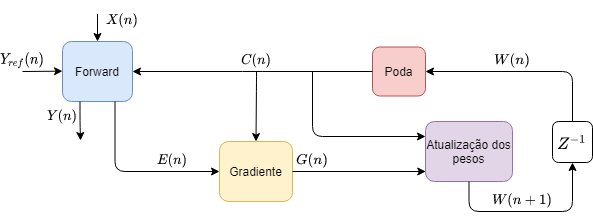
\includegraphics[width=0.7\textwidth, keepaspectratio=true]{figuras/diagram.png}
	\centering
	\caption[Diagrama de loop de aprendizado do \textit{pruning-aware}]{Diagrama de loop de aprendizado do \textit{pruning-aware}}
	\fonte{Elaborada pela autor.}
	%\label{fig:sharpe}
\end{figure}

A cada iteração do loop de aprendizado, foi contabilizada a quantidade de pesos que são removidos e, após isso, foi calculada a esparsidade do modelo, ou seja, a porcentagem de pesos insignificantes da rede. A análise da eficácia da poda é medida a partir da diferença entre as acurácias de de inferência entre o modelo sem compressão e o modelo com compressão.

\begin{figure}[H]
    %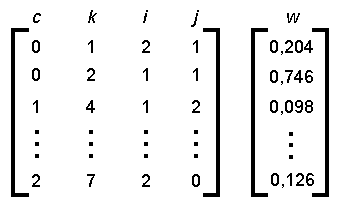
\includepdf[pages=-, width=6cm]{figuras/figx.pdf}
	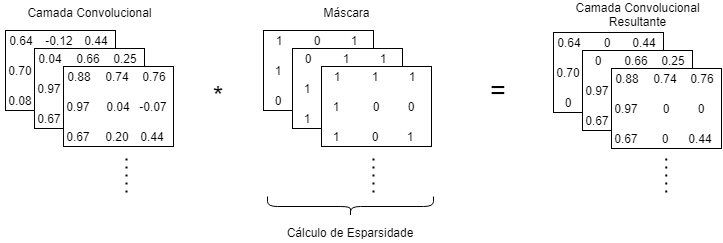
\includegraphics[width=0.8\textwidth, keepaspectratio=true]{figuras/tfmul.png}
	\centering
	\caption[Processo de remoção de pesos na camada convolucional]{Processo de remoção de pesos na camada convolucional}
	\fonte{Elaborada pela autor.}
	%\label{fig:sharpe}
\end{figure}

A remoção dos pesos foi realizada a partir da criação de uma máscara, com o mesmo formato da camada do modelo em análise. Cada índice da máscara é preenchido com zero ou um a depender da magnitude do peso associado na camada. Caso seu peso seja menor que o limiar definido, seu índice será zero, caso contrário será 1. A partir da multiplicação entre a camada e a máscara, é obtido como resultado a camada com os pesos a serem removidos e o valor da esparsidade a partir da contagem de pesos zerados. A figura 10 ilustra como funciona o processo de remoção de pesos. As Figuras 12 e 13 mostram o resultado da remoção dos pesos na segunda camada convolucional do modelo. Como pode ser visto na Tabela 2, a segunda camada convolucional possui 18.496 parâmetros, portanto, nesse exemplo, apenas 2.858 parâmetros possuem pesos significativos.




\begin{figure}[H]
    %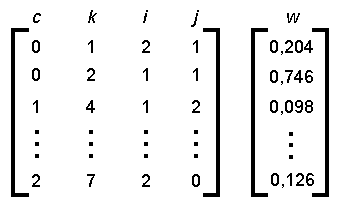
\includepdf[pages=-, width=6cm]{figuras/figx.pdf}
	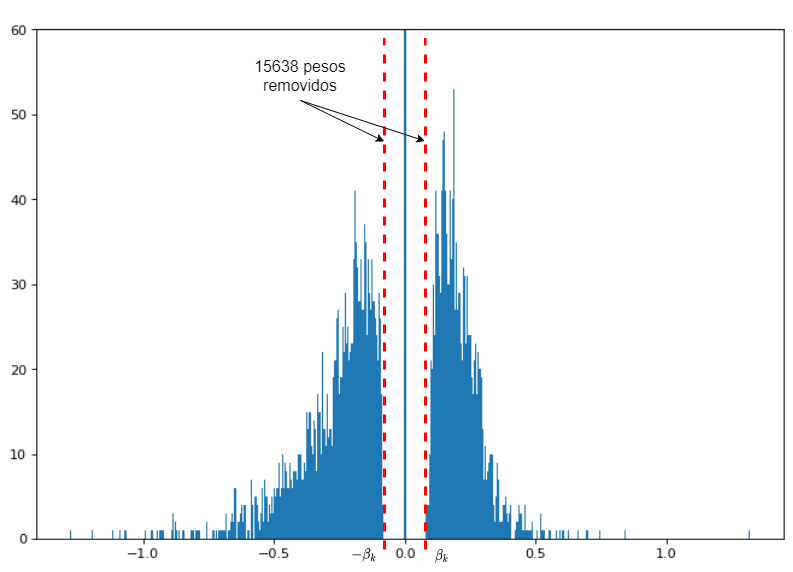
\includegraphics[width=0.65\textwidth, keepaspectratio=true]{figuras/antes (1).png}
	\centering
	\caption[Histograma de pesos da segunda camada convolucional antes da poda]{Histograma de pesos da segunda camada convolucional antes da poda}
	\fonte{Elaborada pela autor.}
	%\label{fig:sharpe}
\end{figure}

\begin{figure}[H]
    %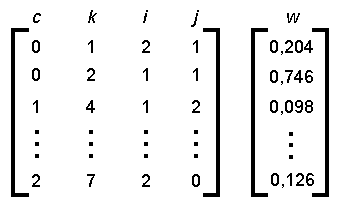
\includepdf[pages=-, width=6cm]{figuras/figx.pdf}
	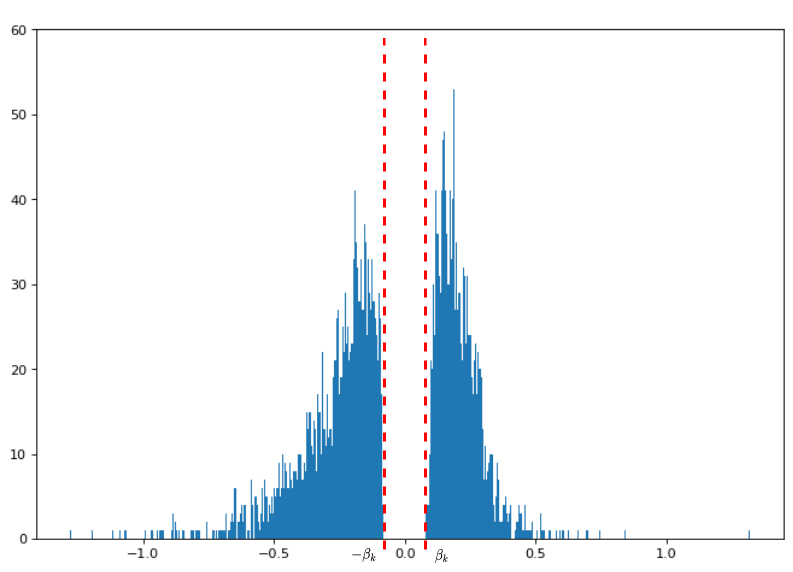
\includegraphics[width=0.65\textwidth, keepaspectratio=true]{figuras/depois.png}
	\centering
	\caption[Histograma de pesos da segunda camada convolucional depois da poda]{Histograma de pesos da segunda camada convolucional depois da poda}
	\fonte{Elaborada pela autor.}
	%\label{fig:sharpe}
\end{figure}

\subsection{Modelo e hiper-parâmetros} \label{secao12}
O processo de treinamento foi realizado sete vezes, variando em $\alpha$ = 0,00, $\alpha$ = 0,25, $\alpha$ = 0,50, $\alpha$ = 0,75, $\alpha$ = 1,00, $\alpha$ = 1,25 e $\alpha$ = 1,50. A função utilizada para cáculo das perdas foi a Sparse Categorical Corossentropy e a função do otimizador utilizada foi Adam. Em todos os experimentos, a estrutura da rede foi criada da seguinte forma:

\begin{enumerate}
   \item Camada de entrada de 32x32x3;
   \item Camada convolucional com 32 kernels de 3x3, sem padding, stride igual a 1 e função de ativição relu;
   \item Camada convolucional com 64 kernels de 3x3, sem padding, stride igual a 1 e função de ativição relu;
   \item Camada de Max-pooling de 2x2, stride igual a 2;
   \item Camada convolucional com 128 kernels de 3x3, sem padding, stride igual a 1 e função de ativição relu;
   \item Camada convolucional com 128 kernels de 3x3, sem padding, stride igual a 1 e função de ativição relu;
   \item Camada de Max-pooling de 2x2, stride igual a 2;
   \item Camada totalmente conectada com 256 neurônios e função de ativação relu;
   \item Camada totalmente conectada com 128 neurônios e função de ativação relu;
   \item Camada de saída para 10 classes com função de ativação softmax.
\end{enumerate}

A tabela 2 mostra a quantidade de parâmetros de cada camada e também de todo o modelo.

\begin{table}[H]
    \centering
    \begin{tabular}{ |p{4cm}|p{3cm}|  }
 %\hline
 %\multicolumn{2}{|c|}{Estrutura da rede utilizada} \\
 \hline
 Tipo de Camada&Quantidade de parâmetros \\
 \hline
    Convolucional 2D        &896    \\
    Convolucional 2D        &18.496    \\
    Max Pooling 2D          &0    \\
    Convolucional 2D        &73.856    \\
    Convolucional 2D        &147.584    \\
    Max Pooling 2D          &0    \\
    Flatten                 &0    \\
    Dense                   &819.456    \\
    Dense                   &32.896    \\
    Dense                   &1.290    \\
    
 \hline
 \multicolumn{2}{|c|}{Total de 1.094.474 parâmetros} \\
 \hline
\end{tabular}
    \caption{Quantidade de parâmetros da rede}
    \label{tab:my_label}
\end{table}












%\subsection{Análise em hardware} \label{section13}

%Após o processo de aprendizagem com compressão, o modelo resultante foi desenvolvido em um hardware de baixo consumo. Para isso, foram feitas algumas modificações no formato do modelo. Foi criado uma matriz armazenando apenas os índices e pesos significativos de cada camada e um vetor contendo o valor dos pesos de forma que uma linha da matriz represente os índices do peso da mesma linha do vetor de pesos. A figura 5 apresenta um exemplo para uma camada convolucional, com \textit{c} representando o canal, \textit{k} representando o \textit{kernel} (filtro), \textit{i} e \textit{j} representando o linha e coluna do peso no kernel e \textit{w} como peso.



%\subsection{Validação} \label{section14}
%Para validar se realmente houve uma diminuição da necessidade do esforço computacional no hardware, primeiro, foi contabilizado a quantidade de pulsos de clock necessários para uma simples operação matemática de multiplicação e soma. Em seguida, foi contabilizado a quantidade de operações numéricas que devem ser realizadas pelo microcontrolador em todo o modelo de acordo com sua esparsidade. Após isso, foi verificado a quantidade de pulsos de clock necessários para que uma certa amostra passe por todo modelo. Por fim, foi verificado se a quantidade de pulsos de clock para operações em todo o modelo estava de acordo com a prevista pela multiplicação entre a quantidade de clocks para uma única operação e a quantidade de operações a serem realizadas no modelo.

%Use \textit{labels} para criar links para as seções, como \autoref{secao1}.

%\lipsum[5-8]


\section{Dataset} \label{secao2}

O dataset escolhido para esse trabalho chama-se CIFAR-10, que consiste em 60 mil imagens coloridas com 3 canais (RGB) de 32x32 pixels divididas em 10 classes, com 6 mil imagens de cada classe. O dataset é dividido em 50 mil imagens para treino e 10 mil para inferência. 

\begin{figure}[H]
    %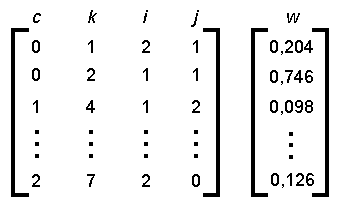
\includepdf[pages=-, width=6cm]{figuras/figx.pdf}
	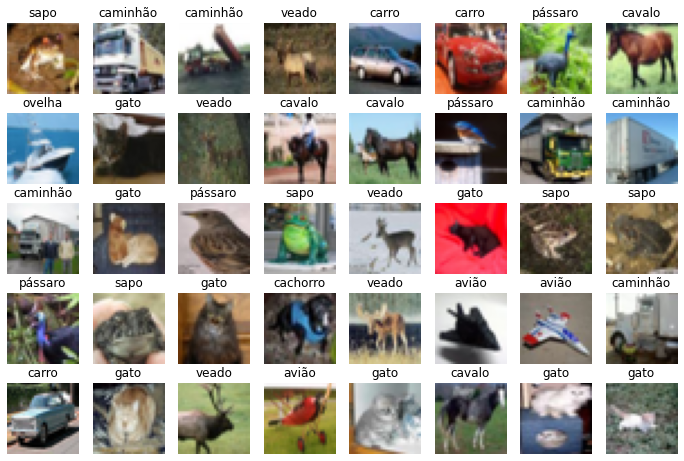
\includegraphics[width=0.7\textwidth, keepaspectratio=true]{figuras/cifar10ex.png}
	\centering
	\caption[Amostras do dataset CIFAR-10]{Amostras do dataset CIFAR-10}
	\fonte{Elaborada pela autor.}
	%\label{fig:sharpe}
\end{figure}




As 10 classes são: avião, automóvel, pássaro, gato, veado, cachorro, sapo, cavalo, barco e caminhão. As classes são exclusivas entre si, ou seja, não há sobreposição entre automóveis e caminhões. A classe de automóveis inclui apenas sedans, SUV's e carros de pequeno porte. A classe de caminhão inclue apenas caminhões grandes, excluindo pickups. A Figura 14 apresenta algumas amostras do dataset.